\section{Implementierungsphase}
	
	Ziel:				
	\begin{itemize}
		\item Leistungssteigerung durch \textbf{Parallelität}
	\end{itemize}
	
	\subsection{Grundlagen der Parallelität}
		
		\begin{itemize}
			\item Architekturstile:
			\begin{itemize}
				\item \textbf{Gemeinsamer Speicher} (Shared memory)
				\begin{itemize}
					\item CPUs haben \underline{einen} Speicher
				\end{itemize}
				\item Verteilter Speicher
				\begin{itemize}
					\item CPU hat eigenen Speicher
				\end{itemize}
			\end{itemize}
		\end{itemize}
				
		\begin{center}
			\begin{tabular}{c|c}
				Prozess                                             & Kontrollfaden (Thread) \\
				\hline
				- Aufgabe eines Programms                           & - Leichtgewichtige Aufgabe eines Prozesses \\
				$\Rightarrow$ \textbf{Durch Betriebssystem erzeugt} & - Greift auf \textbf{Daten des Prozess} zu \\
			\end{tabular}
		\end{center}
		
	\subsection{Parallelität in Java}
			
		\subsubsection{Erzeugen von Kontrollfäden}
					
			\begin{itemize}
				\item Mit Hilfe von:
				\begin{itemize}
					\item Interface \textbf{Runnable}
					\item Klasse \textbf{Thread}
				\end{itemize}
				\newpage
				\item Skizzierter Ablauf:			
			\end{itemize}			
			\begin{center}
				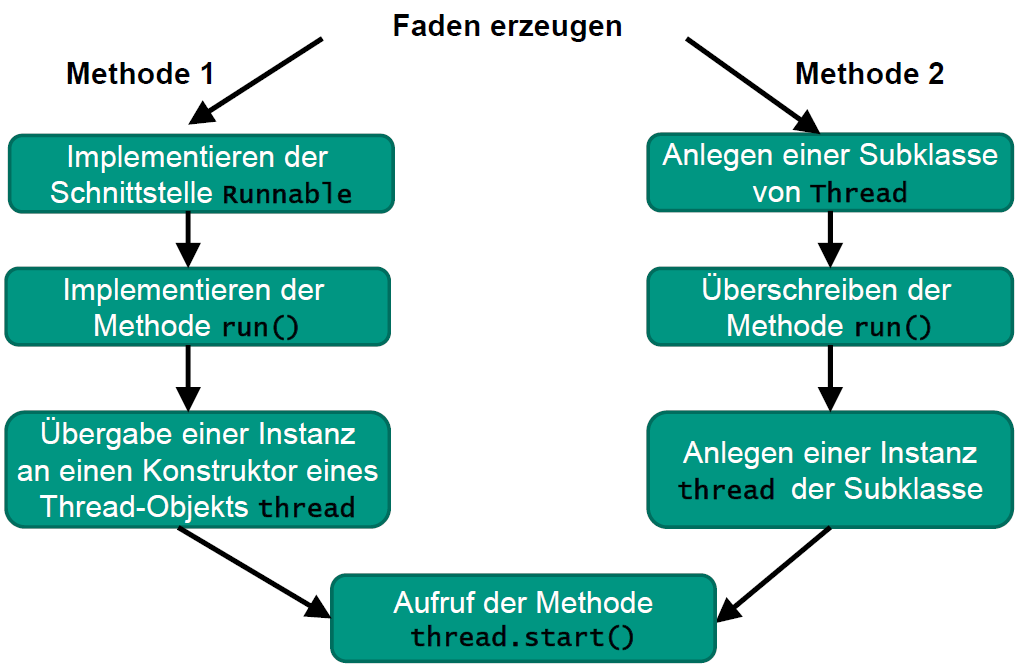
\includegraphics[width=0.7\textwidth]{../images/ablaufParallelitaetJava.png}
			\end{center}
						
			\begin{itemize}
				\item Runnable vs. Thread:
				\begin{itemize}
					\item \textbf{Bessere Modularisierung} mit Runnable
					\begin{itemize}
						\item \textbf{Weniger Overhead} durch Kapselung
						\item Aufgabe kann \textbf{über Netzwerk versendet} werden (\textbf{serialisierbar})
					\end{itemize}
				\end{itemize}
			\end{itemize}
			
		\subsubsection{Konstrukte zum Schützen kritischer Abschnitte}
			
			\begin{itemize}
				\item Koordination von:
				\begin{itemize}
					\item \textbf{Wechselseitigem Ausschluss}
					\begin{itemize}
						\item Eine Aktivität gleichzeitig!
					\end{itemize}
					\item \textbf{Warten auf Ereignisse/Benachrichtigungen}
					\item \textbf{Unterbrechungen}
					\begin{itemize}
						\item Aktivität wartet auf ein (nicht) eintretendes Ereignis
					\end{itemize}
				\end{itemize}
				\newpage
				\item \underline{Wechselseitiger Ausschluss}
				\begin{itemize}
					\item Bei \textbf{gleichzeitigem Datenzugriff} kann es zu \textbf{Wettlaufsituationen} (race conditions) kommen:
					\begin{itemize}
						\item \textbf{Monitor} besetzt Aktivität bis zum Ende mit:
						\begin{itemize}
							\item \textbf{enter()}
							\item \textbf{exit()}
						\end{itemize}
						\item Synchronisierung nach gleichem Prinzip mit:
						\begin{itemize}
							\item \textbf{synchronized (obj)}
							\item \textbf{synchronized void foo()}
						\end{itemize}
					\end{itemize}
					\item Monitor:
				\end{itemize}		
				\begin{center}
					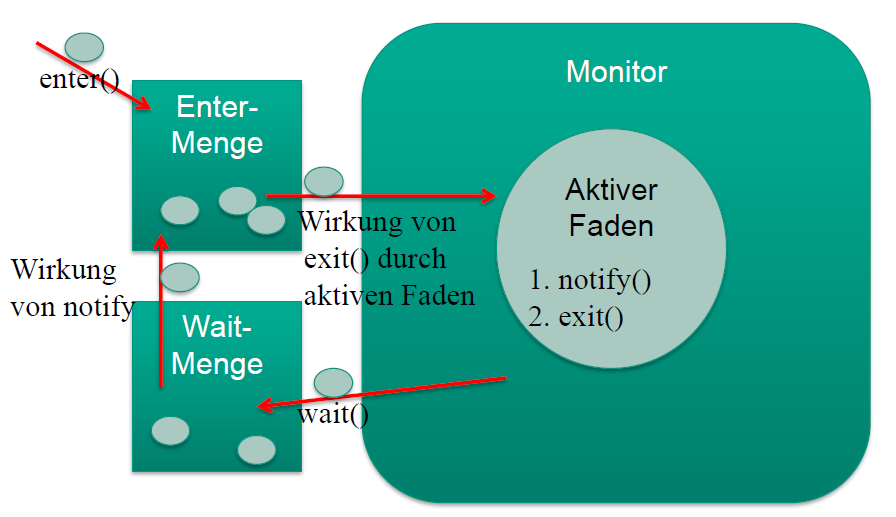
\includegraphics[width=0.8\textwidth]{../images/monitor.png}
				\end{center}				
				\item \underline{Warten auf Ereignisse/Benachrichtigungen}
				\begin{itemize}
					\item Überprüfung, dass nur eine Aktivität gleichzeitig läuft, reicht nicht!
					$\Rightarrow$ \textbf{Warteschlange} spielt eine Rolle!
					\newpage
					\item \underline{Methoden:}
					\begin{itemize}
						\item wait(), notify(), notifyAll() nur im \textbf{synchronized-Block}!
						
						$\Rightarrow$ Monitor ist \dq this\dq und \underline{kann weggelassen} werden
						\newline
						$\Rightarrow$ Falls \underline{nicht} im synchronized-Block: \textbf{IllegalMonitorStateException}
					\end{itemize}
					\item wait():
					\begin{itemize}
						\item Setzt Faden in \textbf{Wartezustand bis Signal} eintritt
											
						\color{red}{$\Rightarrow$ IMMER in einer Schleife!}
						\newline							
						\color{red}{$\Rightarrow$ Bedingung VOR und NACH dem Warten prüfen!}
					\end{itemize}
					\item notify(), notifyAll():
					\begin{itemize}
						\item Schicken \textbf{Signale an wartende Aktivitäten}
													
						\color{red}{$\Rightarrow$ Sicher ist nur: notifyAll()}
					\end{itemize}
				\end{itemize}
				\item \underline{Unterbrechnungen}
				\begin{itemize}
					\item Wie \underline{beendet} man Aktivitäten, die auf \underline{nicht mehr eintreffende} Signale warten?
					$\Rightarrow$ Durch \textbf{interrupt()}
					\item Die Methode \textbf{wait()} kann auch eine \textbf{InterruptedException} werfen!
				\end{itemize}
				\item \underline{Verklemmungen (Deadlocks)}
				\begin{itemize}
					\item \textbf{Semaphore}, die mit \underline{Anzahl an Genehmigungen} initialisiert werden
					\begin{itemize}
						\item \textbf{acquire():} Blockiert bis Genehmigung verfügbar und dann Genehmigungen--
						\item \textbf{release():} Genehmigungen++
					\end{itemize}
					\item \textbf{CyclicBarrier}, die \underline{Gruppen von Fäden} synchronisiert
					\begin{itemize}
						\item Fäden rufen \textbf{await()} auf, die so lange blockiert, \underline{bis alle Fäden warten}
					\end{itemize}
				\end{itemize}
			\end{itemize}
				
		\newpage
		\subsubsection{Bewertung von parallelen Algorithmen}
					
			\begin{itemize}
				\item \textbf{Beschleunigung:}
				\begin{itemize}
					\item {\LARGE ${S}{\left(p\right)}=\frac{T\left(1\right)}{T\left(p\right)}$}
					\item ${S}{\left(p\right)}$ = Angabe, wie viel schneller mit p Prozessoren
				\end{itemize}
				\item \textbf{Effizienz:}
				\begin{itemize}
					\item {\LARGE ${E}{\left(p\right)}=\frac{T\left(1\right)}{p\cdot T\left(p\right)}=\frac{{S}{\left(p\right)}}{p}$}
					\item ${E}{\left(p\right)}$ = Anteil an Ausführungszeit der nützlich verrichteten Arbeit
					\begin{itemize}
						\item \underline{Ideal:} ${S}{\left(p\right)} = {p}$ oder ${E}{\left(p\right)} = {1}$
					\end{itemize}
				\end{itemize}
				\item \textbf{Gesamtlaufzeit:}
				\begin{itemize}
					\item {\LARGE ${T}{\left(p\right)} = \sigma + \frac{\pi}{{p}}$}
					\item $\sigma$ = Zeit für Ausführung des sequentiellen Teils
					\item $\pi$ = Zeit für die sequentielle Ausführung des parallelen Teils
					\item ${p}$ = Anzahl an CPUs
				\end{itemize}
				\item \textbf{Amdahl'sches Gesetz:}
				\begin{itemize}
					\item {\LARGE ${S}{\left(p\right)} \le \frac{1}{f}$} mit {\LARGE ${f} = \frac{\sigma}{\sigma + \pi}$}
				\end{itemize}
			\end{itemize}